\documentclass{article}

\usepackage{hyperref}
\usepackage[utf8]{inputenc}
\usepackage{graphicx} % Required for the inclusion of images
\usepackage{amsmath} % Required for some math elements 
\usepackage[utf8]{inputenc}
\usepackage[english]{babel}
\newtheorem{theorem}{Theorem}
\newtheorem{corollary}{Corollary}[theorem]
\newtheorem{lemma}[theorem]{Lemma}

%TODO follow the instructions on http://workspace.nottingham.ac.uk/display/CompSci/Procedure+for+PhD+Annual+Reviews

% A written report that contains the following sections. There is no specific requirement on formatting but it should be well-presented and proof-read to ensure it is a piece of high-quality academic writing. As guidance, the whole report including the appendix should normally be around 8000-10000 words in length.

%TODO Current title of PhD project, Whether it is a first, second or third annual review report, word count, student name, student ID, names of supervisors, initial registration date, expected date for entering thesis pending stage, expected date for thesis submission.
\title{1st Year Report \\ Pure Functional Methods in \\ Agent-Based Modelling \& Simulation} % Title

\author{Jonathan \textsc{Thaler} \\ jonathan.thaler@nottingham.ac.uk} % Author name

\date{\today} % Date for the report

\begin{document}
\maketitle % Insert the title, author and date

% If you wish to include an abstract, uncomment the lines below
\begin{abstract}
A succinct and concise summary (250 words maximum) of the report contents and presented on a single page.

So far specifying Agent-Based Models and implementing them as an Agent-Based Simulation (ABS) is done using object-oriented methods like UML and object-oriented programming languages like Java. The reason for this is that until now the concept of an agent was always understood to be very close to, if not equals to - which it is not - the concept of an object. Therefore, the reasoning goes, object-oriented methods and languages should fit themselves naturally to specify and implement agent-based simulations. In this PhD Thesis we fundamentally challenge this assumption by investigating how Agent-Based Models and Simulations can be specified and implemented using pure functional methods and programming in Haskell and what the benefits are. We will show that the implicit assumption that an Agent is \textit{about equal to} an Object is not correct and leads to many implicit assumptions in object-oriented implementations of Agent-Based Simulation (ABS). When implementing ABS in Haskell these implicit assumptions become explicit and challenge the fundamental assumptions about ABS and Agents. We present these implicit assumption in an explicit way by approaching it through programming, type-theory and category-theory to further deepen the concepts and methods in the field of Agent-Based Modelling \& Simulation. We also think that the major benefit of implementing ABS in Haskell is the potential for an unprecedented approach of formal validation \& verification of an Agent-Based Model and its implementation. Due to the declarative nature of pure functional programming in Haskell it is possible to implement an EDSL for ABS which ideally results in code which looks like specification thus closing the gap between specification and implementation because the specification is already the code. For validation we want to pursue testing through QuickCheck.

In this report I discuss the research conducted to far, present the open problems together with an in-depth literature review. An outline for the research of the following 2 years is given and the aims.
\end{abstract}

%TODO Contents Page Main headings with page numbers.

\section{Introduction}
There exists a large number of simulation packages which allow the convenient creation of System Dynamics simulations by straight-forward visual diagram creation. One simply creates stocks and flows, connects them, specifies the flow-rates and initial parameters and then runs the model. An example for such a visual diagram creation in the simulation package AnyLogic can be seen in Figure \ref{fig:sir_stockflow_diagram}.

\begin{figure}
	\centering
	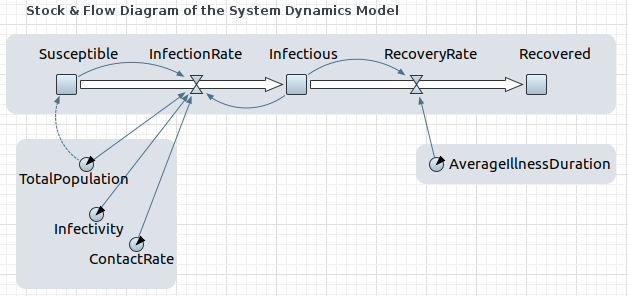
\includegraphics[width=.5\textwidth, angle=0]{./fig/SIR_SD_STOCKFLOW_DIAGRAMM.png}
	\caption{Visual System Dynamics Diagram of the SIR model in AnyLogic Personal Learning Edition 8.3.1.}
	\label{fig:sir_stockflow_diagram}
\end{figure}

Still, implementing System Dynamics directly in code is not as straight forward and involves numerical integration which can be quite tricky to get right. Thus, the aim of this paper is to look into how System Dynamics models can be implemented in code correctly without the use of a simulation package. We use the well known SIR model \cite{kermack_contribution_1927} from epidemiology to demonstrate our approach.

Our language of choice is Haskell because it emphasises a declarative programming style in which one describes \textit{what} instead of \textit{how} to compute. Further it allows to rule out interference with non-deterministic influences or side-effects already at compile-time. This is of fundamental importance for System Dynamics because it behaves completely deterministic and involves no stochastics or non-determinism whatsoever. Also, we make use of Functional Reactive Programming which allows to express continuous-time systems in a functional way. 

We show that by this approach we can arrive at correct-by-construction implementations of System Dynamic models. This means that the correctness of the code is obvious because we have closed the gap between the model specification and its implementation. Thus, the contribution of the paper is the demonstration of how to implement correct-by-construction System Dynamics simulations using Haskell and Functional Reactive Programming.

\chapter{Literature Review}
In this we present a literature-review which is driven by the motivating questions from the introduction. We present relevant sources which pose possible answers and directions of approaches to the posed questions. Based upon this information, in the next chapter we will select our directions and methods for our research, identify the gap we have to bridge with our PhD research and our objectives in achieving to close the gap.

\subsection{Actor Model}
The Actor-Model, a model of concurrency, was initially conceived by Hewitt in 1973 \cite{hewitt_universal_1973} and refined later on \cite{hewitt_what_2007}, \cite{hewitt_actor_2010}. It was a major influence in designing the concept of agents and although there are important differences between actors and agents there are huge similarities thus the idea to use actors to build agent-based simulations comes quite natural. The theory was put on firm semantic grounds first through Irene Greif by defining its operational semantics \cite{greif_semantics_1975} and then Will Clinger by defining denotational semantics \cite{clinger_foundations_1981}. In the seminal work of Agha \cite{agha_actors:_1986} he developed a semantic mode, he termed \textit{actors} which was then developed further \cite{agha_foundation_1997} into an actor language with operational semantics which made connections to process calculi and functional programming languages (see both below). 

An actor is a uniquely addressable entity which can \textit{in response to a message}
\begin{itemize}
	\item Send an arbitrary number (even infinite) of messages to other actors.
	\item Create an arbitrary number of actors.
	\item Define its own behaviour upon reception of the next message.
\end{itemize}

In the actor model theory there is no restriction on the order of the above actions and so an actor can do all the things above in parallel and concurrently at the same time. This property and that actors are reactive and not pro-active is the fundamental difference between actors and agents, so an agent is \textit{not} an actor. There have been a few attempts on implementing the actor model in real programming languages where the most notable are Erlang and Scala.

\subsubsection{Erlang}
The programming-model of actors \cite{agha_actors:_1986} was the inspiration for the Erlang programming language which was created in the 80s by Eriksson for developing distributed high reliability software in telecommunications. There exists very little research in using Erlang for ABS \cite{varela_modelling_2004}, \cite{di_stefano_using_2005}, \cite{di_stefano_exat:_2007}, \cite{sher_agent-based_2013}, \cite{Bezirgiannis2013}. TODO: short explanation of what they are doing

\subsubsection{Scala}
Scala is a multi-paradigm language which also comes with an implementation of the actor-model as a library which enables to do actor-programming in the way of Erlang. It was developed in 2004 and became popular in recent years due to the increased availability of multi-core CPUs which emphasised the distributed, parallel and concurrent programming for which the actor-model is highly suited.
As for Erlang, there exists even less research in using Scala \& Actors for ABS TODO: cite.  TODO: short explanation of what they are doing

\subsection{Process Calculi}
pi calculus,...
there is a paper on actor model \& pi-calculus

TODO: \cite{padget_pi-calculus_1998}

TODO: check my folders with print-outs and add them as references but dont discuss them

\section{Pure Functional Programming}
In his 1977 ACM Turing Award Lecture, John Backus \footnote{One of the giants of Computer Science, a main contributor to Fortran - an imperative programming language.} fundamentally critizied imperative programming for its deep flaws and proposed a functional style of programming to overcome the limitations of imperative programming \cite{backus_can_1978}. The main criticism is its use of \textit{state-transition with complex states} and the inherent semantics of state-manipulation. In the end an imperative program consists of a number of assign-statements resulting in side-effects on global mutable state which makes reasoning about programs nearly impossible. Backus proposes the so called \textit{applicative} computing, which he termes \textit{functional programming} which has its foundations in the Lambda Calculus \cite{church_calculi_1941}. The main idea behind it is that programming follows a declarative rather than an imperative style of programming: instead of describing \textit{how} something is computed, one describes \textit{what} is computed. This concept abandons variables, side-effects and (global) mutable state and resorts to the simple core of function application, variable substitution and binding of the Lambda Calculus. Although possible and an important step to understand the very foundations, one does not do functional programming in the Lambda Calculus \cite{michaelson_introduction_2011}, as one does not do imperative programming in a Turing Machine. 
In our thesis we selected Haskell as our functional programming language. \footnote{Although we did a bit of research using Scala (a mixed paradigm functional language) in ABS (see Appendix \ref{app:frABS}), we deliberately ignored other functional languages as it is completely out-of-scope of this thesis to do an in-depth comparison of functional languages for their suitability to implement ABS.}. The paper of \cite{hudak_history_2007} gives a comprehensive overview over the history of the language, how it developed and its features and is very interesting to read and get accustomed to the background of the language. A widely used introduction to programming in Haskell is \cite{hutton_programming_2016}. The main points why we decided to go for Haskell are

\begin{itemize}
	\item Pure, Lazy Evaluation, Higher-Order Functions and Static Typing - these are the most important points for the decision as they form the very foundation for composition, correctness, reasoning and verification. 
	\item Real-World applications - the strength of Haskell has been proven through a vast amount of highly diverse real-world applications \footnote{\url{https://wiki.haskell.org/Applications_and_libraries}} \cite{hudak_history_2007} and is applicable to a number of real-world problems \cite{osullivan_real_2008}.
	\item Modern - Haskell is constantly evolving through its community and adapting to keep up with the fast changing field of computer science e.g. parallelism \& concurrency.
	\item In-house knowledge - the School of Computer Science of the University of Nottingham has a large amount of in-house knowledge in Haskell which can be put to use and leveraged in my thesis.
\end{itemize}

It seems that we are on the right track with pure functional programming in answering the questions in the motivation as it promises to solve all the issues raised in these questions. We will now investigate whether this is really the case by looking into relevant literature. 

The main conclusion of the classical paper \cite{hughes_why_1989} is that \textit{modularity} is the key to successful programming and can be achieved best using higher-order functions and lazy evaluation provided in functional languages like Haskell. The author argues that the ability to divide problems into sub-problems depends on the ability to glue the sub-problems together which depends strongly on the programming-language. He shows that laziness and higher-order functions are in combination a highly powerful glue and identifies this as the reason why functional languages are superior to structure programming. Another property of lazy evaluation is that it allows to describe infinite data-structures, which are computed as currently needed. This makes functions possible which produce an infinite stream which is consumed by another function - the decision of \textit{how many} is decoupled from \textit{how to}.

In the paper \cite{wadler_essence_1992} Wadler describes Monads as the essence of functional programming (in Haskell). Originally inspired by monads from category-theory (see below) through the paper of Moggi \cite{moggi_computational_1989}, Wadler realized that monads can be used to structure functional programs \cite{wadler_comprehending_1990}. A pure functional language like Haskell needs some way to perform impure (side-effects) computations otherwise it has no relevance for solving real-world problems like GUI-programming, graphics, concurrency,... . This is where monads come in, because ultimately they can be seen as a way to make effectful computations explicit \footnote{This is seen as one of the main impacts of Haskell had on the mainstream programming \cite{hudak_history_2007}}. 
In \cite{wadler_essence_1992} Wadler shows how to factor out the error handling in a parser into monads which prevents code to be cluttered by cross-cutting concerns not relevant to the original problem. Other examples Wadler gives are the propagating of mutable state, (debugging) text-output during execution, non-deterministic choice. Further applications of monads are given in \cite{wadler_essence_1992}, \cite{wadler_monads_1995}, \cite{wadler_how_1997} where they are used for array updating, interpreting of a language formed by expressions in algebraic data-types, filters, parsers, exceptions, IO, emulating an imperative-style of programming. This seems to be exactly the way to go, tackling the problems mentioned in the introduction: making data-flow explicit, allowing to factor out cross-cutting concerns and encapsulate side-effects in types thus making them explicit.

The concept of monads was further generalized by Hughes in the concept of arrows \cite{hughes_generalising_2000}. The main difference between Monads and Arrows are that where monadic computations are parameterized only over their output-type, Arrows computations are parametrised both over their input- and output-type thus making Arrows more general. In \cite{hughes_programming_2005} Hughes gives an example for the usage for Arrows in the field of circuit simulation. Streams are used to advance the simulation in discrete steps to calculate values of circuits thus the implementation is a form of \textit{discrete event simulation} - which is in the direction we are heading already with ABS. As will be shown below, the concept of arrows is essential for Functional Reactive Programming a potential way to do ABS in pure functional programming.

One of the most compelling example to utilize pure functional programming is the reporting of \cite{hudak_haskell_1994} where in a prototyping contest of DARPA the Haskell prototype was by far the shortest with 85 lines of code (LoC) as compared to the C++ solution with 1105 LoC. The remarkable thing is that the Jury mistook the Haskell code as specification because its approach was to implement a small embedded domain specific language (EDSL) to solve the problem - this is a perfect proof how close an EDSL can get to a specification. When implementing an EDSL one develops and programs primitives e.g. types and functions in a host language (embed) in a way that they can be combined. The combination of these primitives then looks like a language specific to a given domain. The ease of development of EDSLs in pure functional programming is also a proof of the superior extensibility and composability of pure functional languages over object-orientation and is definitely one of its major strength. The classic paper \cite{henderson_functional_1982} gives a wonderful way of constructing an EDSL to denotationally construct a picture reminiscent of the works of Escher.
A major strength of developing an EDSL is that one can reason about and do formal verification. A nice introduction how to do reasoning in Haskell is given in \cite{hutton_tutorial_1999}. Also the testing-library QuickCheck \cite{claessen_quickcheck:_2000}, \cite{claessen_testing_2002} defines an EDSL which allows to formulate a specification in the QuickCheck- EDSL and domain-EDSL and test the code against this specification - testing code happens by writing formal specifications which is the very heart of verification. 
It seems that in EDSL we have found a way to tackle the problem of verification and close the gap between specification and implementation at least conceptually - whether this is really possible will be subject of the research conducted in the thesis.

\subsection{ABS}
The amount of research on using the pure functional paradigm using Haskell in the field of ABS has been moderate so far. Most of the papers look into how agents can be specified using the belief-desire-intention paradigm \cite{de_jong_suitability_2014}, \cite{sulzmann_specifying_2007}, \cite{jankovic_functional_2007}. A library for Discrete Event Simulation (DES) and System Dynamics (SD) in Haskell called \textit{Aivika 3} is described in \cite{sorokin_aivika_2015}. It comes with very basic features for ABS but only allows to specify simple state-based agents with timed transitions.
\cite{jankovic_functional_2007} which discuss using functional programming for DES mention the paradigm of functional reactive programming (FRP) to be very suitable to DES. \cite{schneider_towards_2012} and \cite{vendrov_frabjous:_2014} present a domain-specific language for developing functional reactive agent-based simulations. This language called FRABJOUS is human readable and easily understandable by domain-experts. It is not directly implemented in FRP/Haskell but is compiled to Yampa code - a FRP library for Haskell - which they claim is also readable. It seems that FRP is a promising approach to ABS in Haskell, an important hint we will follow in the section below.

Tim Sweeney, CTO of Epic Games gave an invited talk in which he talked about programming languages in the development of game-engines and scripting of game-logic \cite{sweeney_next_2006}. Although the fields of games and ABS seem to be very different, in the end they have also very important similarities: both are simulations which perform numerical computations and update objects in a loop either concurrently or sequential \footnote{Gregory \cite{gregory_game_2018} defines computer-games as \textit{soft real-time interactive agent-based computer simulations}}. In games these objects are called \textit{game-objects} and in ABS they are called \textit{agents} but they are conceptually the same thing. The two main points Sweeney made were that dependent types could solve most of the run-time failures and that parallelism is the future for performance improvement in games. He distinguishes between pure functional algorithms which can be parallelized easily in a pure functional language and updating game-objects concurrently using software transactional memory (STM).

The thesis of \cite{bezirgiannis_improving_2013} constructs two frameworks: an agent-modelling framework and a DES framework, both written in Haskell. They put special emphasis on parallel and concurrency in their work. The author develops two programs with strong emphasis on parallelism: HLogo which is a clone of the NetLogo agent-modelling framework and HDES, a framework for discrete event simulation.

Although probably the most important selling point of a pure functional language is its ease of parallelizing code due to lack of side-effects \cite{peyton_jones_concurrent_1996}, \cite{osullivan_real_2008}, \cite{jones_tutorial_2009}, \cite{marlow_parallel_2013} we don't go into this direction in our thesis and consider this just to be a by-product which luckily just falls out of the language itself \footnote{We did some research of implementing concurrent agents with STM as proposed by \cite{sweeney_next_2006} and \cite{bezirgiannis_improving_2013} in our research on programming paradigms as can be seen in Appendix \ref{app:paradigms}. We think that STM is probably the single major feature which is \textit{only} possible in a pure functional language because only in a pure functional language with explicit side-effects it is possible to \textit{compose} concurrency.}.

%TODO: this seems all to be focused on MAS
%\url{http://haskell-distributed.github.io/wiki.html} looks good but too big and not well suited for simulations
%\url{https://code.google.com/archive/p/haskellactor/} makes heavy use of IORef and running in IO-Monad, something we deliberately want to avoid to keep the ability to reason about the program.
%TODO: \url{https://github.com/fizruk/free-agent} look into

\subsection{Functional Reactive Programming}
So far we have considered only quite low-level approaches to structuring and composing functional programming: higher-order functions, laziness, monads and arrows. What we need is a programming paradigm built into pure functional programming which we can leverage to implement ABS. As already mentioned above, functional reactive programming (FRP) seems to be a highly promising approach. It is rather a lucky coincidence that Henrik Nilsson, one of the major contributor to the library Yampa, an implementation of FRP, is situated at the School of Computer Science of the University of Nottingham.

FRP is a paradigm for programming hybrid systems which combine continuous and discrete components. Time is explicitly modelled: there is a continuous and synchronous time flow. There have been many attempts to implement FRP in libraries which each has its benefits and deficits. The very first functional reactive language was Fran, a domain specific language for graphics and animation. At Yale FAL, Frob, Fvision and Fruit were developed. The ideas of them all have then culminated in Yampa, the most recent FRP library \cite{nilsson_functional_2002}. The essence of FRP with Yampa is that one describes the system in terms of signal functions in a declarative manner using the EDSL of Yampa. During execution the top level signal functions will then be evaluated and return new signal functions which act as continuations. A major design goal for FRP is to free the programmer from 'presentation' details by providing the ability to think in terms of 'modeling'. It is common that an FRP program is concise enough to also serve as a specification for the problem it solves \cite{wan_functional_2000}.

Yampa has been used in multiple agent-based applications: \cite{hudak_arrows_2003} uses Yampa for implementing a robot-simulation, \cite{courtney_yampa_2003} implement the classical Space Invaders game using Yampa, \cite{nilsson_declarative_2014} implements a Pong-clone, the thesis of \cite{meisinger_game-engine-architektur_2010} shows how Yampa can be used for implementing a Game-Engine, \cite{mun_hon_functional_2005} implemented a 3D first-person shooter game with the style of Quake 3 in Yampa. Note that although all these applications don't focus explicitly on agents all of them inherently deal with kinds of agents which share properties of classical agents: game-entities, robots,... Other fields in which Yampa was successfully used were programming of synthesizers, network routers, computer music development and has been successfully combined with monads \cite{perez_functional_2016}.

This leads to the conclusion that Yampa is mature, stable and suitable to be used in functional ABS. This and the reason that we have the in-house knowledge lets us focus on Yampa. Also it is out-of-scope to do a in-depth comparison of the many existing FRP libraries.

\subsection{Dependent Types}
As already pointed out by Sweeney in \cite{sweeney_next_2006}, dependent types could remove an important class of run-time errors which in the end means that using them allows to push correctness even further because type-invariants are statically checked at compile time. As correctness and verification is our major concern, dependent types seem to be attractive. The papers of \cite{norell_dependently_2009}, \cite{bove_brief_2009} and \cite{bove_dependent_2009} give a good introduction of what dependent types are and how to program with them in Agda, a dependently typed pure functional programming language, closely related to Haskell. For now this approach seems to be too early to follow as we haven't yet laid the basic groundwork: an non-dependently typed pure functional implementation of ABS in Haskell.
%The delicate point is, that programming in Agda becomes a proof-assistant: a proof is then a constructed programm. The work of \cite{ionescu_dependently-typed_2012} which was mentioned in the introduction uses dependent types for proving fundamental theorems in economics. 

\subsection{Foundations in Category-Theory}
With the advent of monads the interest in category-theory surged and it was discovered that many computational concepts can be expressed through category-theory \cite{pierce_basic_1991}, \cite{spivak_category_2014}. Because many concepts of functional programming were put on firm grounds it would be only consequential to find a category-theoretical approach to functional ABS and put its foundations on firm category-theoretical grounds as well. So far only two papers looked into category-theoretical approaches to agent-based models and simulating \cite{beheshti_analyzing_2013}, \cite{lloyd_category-theoretic_2010} but none of them is really satisfying, making this an ideal research topic for the thesis.

%ADOM: Agent Domain of Monads: https://www.haskell.org/communities/11-2006/html/report.html

\subsection{A final word on LISP}
Being the oldest functional programming language and the 2nd oldest high-level programming language ever created, at one point we considered using LISP in our research due to its immensely powerful feature of homoiconicity. The idea was to investigate if this could be made useful for ABS and bring it to a new level. We abandoned this quickly as it would have led to a total different approach. Besides, it would have definitely not solved the issues the questions raised in the introduction because of its imperative nature. Still there exists a paper \cite{kawabe_nepi2programming_2000} which implements a MAS in LISP.

\section{Agent-Based Social Simulation (ABSS)}
The field of social simulation can be traced back to self-replicating von Neumann machines, cellular automata and Conway's Game of Life. The famous Schelling segregation model \cite{schelling_dynamic_1971} is regarded as a pioneering example. The most prominent topics which are explored in social simulation are social norms, institutions, reputation, elections and economics.

Axelrod \cite{axelrod_advancing_1997}, \cite{axelrod_guide_2006} has called social simulation the third way of doing science, which he termed the \textit{generative} approach which is in opposition to the classical inductive (finding patterns in empirical data) and deductive (proving theorems). Thus the generative approach can be seen as a form of empirical research and is a natural environment for studying social and interdisciplinary phenomena as discussed more in-depth in the work of Epstein \cite{epstein_chapter_2006}, \cite{epstein_generative_2012}. He gives a fundamental introduction to agent-based social social simulation and makes the strong claim that \textit{"If you didn't grow it, you didn't explain its emergence"} \footnote{Emergence is treated more in-depth in the Verification \& Validation section.} \footnote{Note the fundamental constructivist approach to social science, which implies that the emergent properties are actually computable. This applies to ACE as well, which can be seen to be its most fundamental difference to general equilibrium theory of neo-classical economics which is non-constructive. When making connections from the simulation to reality (as in validation, see below), constructible emergence raises the question whether our existence is computable or not. When pushing this further, we can conjecture that the future of simulation will be simulated copies of our own existence which potentially allows to simulate \textit{everything}. An interesting treatment of this can be found in \cite{bostrom_are_2003} and \cite{steinhart_theological_2010}.}. Epstein puts much emphasis on the claim that ABSS is indeed a scientific instrument as hypotheses which are investigated are empirical falsifiable: the simulation exhibits the emergent pattern in which case the model is \textit{one} way of explaining it or it simply does not show the emergent pattern, in which case the hypothesis, that the model (the micro-interactions amongst the agents) generates the emergent pattern is falsified \footnote{This is fundamentally following Poppers theory of science \cite{popper_logic_2002}.} - we haven't found an explanation \textit{yet}. So in summary, growing a phenomena is a necessary, but not sufficient condition for explanation \cite{epstein_chapter_2006}.

% NOTE: incorporate this only when there is enough time (and energy) to go through the 3 references cited here
%This raises a number of philosophical questions \cite{frigg_philosophy_2009}, \cite{grune-yanoff_philosophy_2010}, \cite{borrill_agent-based_2011}. Although we don't want to give an in-depth discussion of the questions raised, we want to have a quick look at them as this is a foundational research-proposal for a Doctor in \textit{Philosophy} (Ph.D.).
%TODO: read above papers and give short outline philosophical questions

The first large scale ABSS model which rose to some prominence was the \textit{Sugarscape} model developed by Epstein and Axtell in 1996 \cite{epstein_growing_1996}. Their aim was to \textit{grow} an artificial society by simulation and connect observations in their simulation to phenomenon of real-world societies. The main features of this model are:

\begin{itemize}
	\item Searching, harvesting and consuming of resources.
	\item Wealth and age distributions.
	\item Seasons in the environment and migration of agents.
	\item Pollution of the environment.
	\item Population dynamics under sexual reproduction.
	\item Cultural processes and transmission.
	\item Combat and assimilation.
	\item Bilateral decentralized trading (bartering) between agents with endogenous demand and supply.
	\item Emergent Credit-Networks.
	\item Disease Processes, Transmission and immunology.
\end{itemize}

Because of its essential importance to this field, its complexity, number of features and allowing us to bridge the gap to ACE, we select it as the first of two central models, which will serve as use-case to develop our methods. The idea is to formally specify and then verify the process of bilateral decentralized trading because it is the most complex of the features and connects directly to ACE.

In 2013 Epstein introduced the \textit{Agent\_Zero} model \cite{epstein_agent_zero:_2014} in which the author approaches the generative social sciences from a neurocognitive perspective \footnote{Epstein termed this work Volume III in the triology on generative social science. Volume I is the Sugarscape book mentioned above \cite{epstein_growing_1996}. Volume II is a collection of papers published in the book \cite{epstein_generative_2012} which applied agent-based modelling to the fields of economics, archeology, conflict, epidemiology, spatial games and the dynamics of norms.}.
\textit{Agent\_Zero} is an agent which is endowed with emotional/affective (emotional/gefühlsbezogen), cognitive/deliberative (wahrnehmung/abwägend) and social modules which are all interconnected and interact with each other. Also Agent\_Zero is always part of a social network through which it is influenced by other Agent\_Zero and can influence them. The core behaviour Epstein wants to "grow" in this model is \textit{"the person who feels no aversion to black people, who has never had any direct evidence or experience of black wrongdoing [...], and who yet initiates the lynching"} \footnote{\cite{epstein_agent_zero:_2014}, page 2}. The central concept of the model is the one of \textit{dispositional contagion} which allows to replicate and simulate the following scenarios (amongst others):

\begin{itemize}
	\item Fight vs. Flight
	\item Replicating the Latané-Darley experiment
	\item Growing the 2011 Arab Spring
	\item Jury processes
	\item Prices and seasonal economic cycles
	\item Mutual escalation spirals
\end{itemize}

We select \textit{Agent\_Zero} as our second central model serving as use-case to develop our methods because of its in ABSS and offers a very interesting use-case to apply various networks as presented in the ACE section \footnote{In a recent work \cite{epstein_advancing_2016} Epstein offers a range of new research directions for Agent\_Zero, most notably new interactions, empirical testing, replication of historical episodes and formal axioms for modular agents. We include it for completeness but it does not offer fundamentally new insights to Agent\_Zero neither does it approach the lack of a deeper treatment of the influence of networks in the model.}. As Epstein only looks at a network of three agents, the idea is to investigate the effect of various types of networks as presented in the literature-review section on ACE with much more than three agents on the model.

\subsection{Agent-Based Computational Economics (ACE)}
The field of economics is an immensely vast and complex one with many facets to it \cite{bowles_understanding_2005}. Equilibrium-theory is the very foundation of (micro) economics \cite{colell_microeconomic_1995} and central to the way economists think and approach the dynamics of economic processes. This model requires a central \textit{walrasian} auctioneer which has perfect information and assumes homogeneous, rationally acting agents. The theory then postulates the existence of an equilibrium under given properties but does not give a process or the dynamics how this equilibrium can be approached. 
This notion of equilibrium has always been criticized for being not realistic, making impossible assumptions e.g. perfect information and not being able to provide a process under which this equilibrium is reached \cite{kirman_complex_2010}. The problem is that as soon as more realistic assumptions are made, the solutions become analytically intractable. This is where ACE comes in, as it allows to experimentally approach equilibrium-theory from a more realistic point-of-view by removing the central auctioneer and introducing agents with bounded rationality, local information and restricted interactions over networks \cite{farmer_economy_2009}. 
%look into computable economics book: \url{http://www.e-elgar.com/shop/computable-economics}

Tesfatsion defines ACE as \textit{[...] computational modelling of economic processes (including whole economies) as open-ended dynamic systems of interacting agents.} \url{http://www2.econ.iastate.edu/tesfatsi/ace.htm}. She gives a broad overview \cite{tesfatsion_agent-based_2006} of ACE, discusses advantages and disadvantages and giving the four primary objectives of it which are:

\begin{enumerate}
	\item empirical understanding: why have particular global regularities evolved and persisted, despite the absence of centralized planning and control?
	\item normative understanding: how can agent-based models be used as laboratories for the discovery of good economic designs?
	\item qualitative insight and theory generation: how can economic systems be more fully understood through a systematic examination of their potential dynamical behaviors under alternatively specified initial conditions?
	\item methodological advancement: how best to provide ACE researchers with the methods and tools they need to undertake the rigorous study of economic systems through controlled computational experiments?
\end{enumerate}

She introduces a model called \textit{ACE Trading World} in which she shows how an artificial economy can be implemented without the \textit{Walrasian Auctioneer} but just by agents and their interactions. She gives a detailed mathematical specification in the appendix of the paper which should allow others to implement the simulation. Other works which investigate ACE as a discipline and discuss its methodology are \cite{tesfatsion_agent-based_2002}, \cite{richiardi_agent-based_2007}, \cite{ballot_agent-based_2015}, \cite{blume_introduction_2015}

During the reading we became particularly interested in the dynamics of bilateral decentralized bartering \footnote{The Sugarscape book \cite{epstein_growing_1996}, in footnote 14 on page 104, cites a few introductory works on bilateral bartering with incomplete information which we don't want to repeat here} and emerging networks. The reason for this is that the Sugarscape model \cite{epstein_growing_1996}, mentioned in the previous section on Social Simulation, implements this bilateral decentralized bartering and emerging of credit-networks and looks at the out-of-equilibrium dynamics. This allows us to bridge the gap from ACE to Social Simulation because considerable research in ACE goes into out-of-equilibrium models, which try to find processes which lead to the general equilibrium \cite{gintis_emergence_2006}, \cite{gintis_dynamics_2007}, \cite{arthur_out--equilibrium_2006} and \cite{botta_functional_2011}.

Although not directly subject of this research, to better understand trading and bartering, it is quite useful to have a basic understanding of \textit{Market Microstructure} which deals how real markets work \footnote{A topic we deliberately ignore is the one of \textit{Market Design} which deals with problems real markets face. It is a very hot topic at the moment in economics, having received a number of Nobel-prices e.g. Alvin Roth who wrote an introduction to this topic for the non-expert \cite{roth_who_2015}. In the preparation phase we did quite some reading in this field inspired by \cite{sornette_crashes_2011} and \cite{budish_editors_2015} on the problems caused by High-Frequency Trading (HFT). We were able to find quite a few papers which used ABS to research the benefits and downside of HFT: \cite{wah_latency_2013}, \cite{leal_rock_2016}, \cite{yim_effect_2015}. A broad overview of Market Design using Agent-Based Models is given in \cite{marks_chapter_2006}}. Introductory texts to market microstructure are \cite{harris_trading_2003}, \cite{baker_market_2013} and \cite{lehalle_market_2013}. A highly interesting research using ABS for simulating the NASDAQ market was done in \cite{darley_nasdaq_2007}. The authors where approached by NSDAQ to predict the switching to the decimal system which was enforced by the SEC in April 9th 2001. They implemented an ABS in Java to build relevant models and predicted most of the changes correctly. Other works on using ABS in finance and stock markets are \cite{lebaron_agent-based_2000}, \cite{lebaron_building_2002}, \cite{streltchenko_multi-agent_2005} and \cite{panayi_agent-based_2012}. Another sub-field is autonomous and automated trading agents \cite{mackie-mason_chapter_2006}, \cite{toulis_mertacor:_2006}.

Another topic I am particularly interested in is the one of networks as it was of central focus in my master-thesis TODO:cite on continuous double-auctions in networks. Although this topic is not unique to economics, it has received considerable attention in the last years due to the sub-prime mortgage crisis where contagion through networks was one of the primary reasons for its cause.

TODO: add literature on networks from my masterthesis.
TODO cite Jackson Social and Economic networks, cite easley networks, crowds and markets


\begin{enumerate}
	\item Bilateral decentralized bartering \&  trading
	\item Out-Of-Equilibrium dynamics
	\item Networks
\end{enumerate}

 \footnote{It is of very importance to note that this thesis does not attempt to develop or proof some economic theory. Rather the intention is to use ACE as a use-case to develop the tools and apply them directly to ACE to demonstrate the usefulness and benefit of the new tool.}.

\section{Verification \& Validation of ABS}
Verification \& Validation are, generally speaking, independent processes to check whether a product meets its requirements and fulfills its intended purpose TODO: cite?. Here we focus explicitly on software verification \& validation where we identify \textit{Verification} to be the process of checking whether an implementation matches a given specification without any bugs or missing parts and \textit{Validation} to be the process of checking if the implementation meets high level requirements. TODO: cite?
To put short the difference between verification \& validation is that verification tries to answer "are we building the product right?" and validation "are we building the right product?" \cite{boehm_software_1989}. For (most of) the software built in the industry in well-defined software-development processes with its own quality control and quality assurance to answer these questions is rather straight-forward. Numerous techniques like checklists, software-tests, integration-tests,... have been developed to deal with Verification \& Validation. TODO: cite?

The question is how the above applies to ABS and from reviewing the literature, it becomes evident that in the context of ABS it is a much more difficult challenge and is still open research \footnote{Leigh Tesfatsion has, as part of her internet-presence on ACE, set up a whole site devoted just to this topic where she cites major references \url{http://www2.econ.iastate.edu/tesfatsi/empvalid.htm}. Most of the literature we have investigated  is drawn from there.}. 

In this thesis we aim for replicating both the Sugarscape \cite{epstein_growing_1996} and Agent\_Zero \cite{epstein_agent_zero:_2014} models. In doing so we also perform verification \& validation on these models, or at least on parts of them. Also we aim to develop new methods of verification and validation of ABS based on theses models as use-cases. 

The issue of validation \& verification is also very closely related to the problem of replication. In the paper \cite{wilensky_making_2007} Wilensky discusses the issues with replicating a model and gives advices to modellers what details (e.g. order of events) to publish to support replication of models. They recommend to make pseudo-code publicly available and to converge to a common standard form for model publication in the long run. This is our approach: an EDSL can act both as a pseudo-code specification which is in fact already runnable code and due to its declarative and concise nature can act as a full description.
 
\cite{galan_errors_2009} makes the critical point that the dynamics of a model in ABS are almost always so complex, that the creator of the is not able to exactly explain what the deeper reasons are for them and which aspects of the model are responsible for their exhibition. If this were so, one would not need to resort to simulation. This implies that one can not know in advance what exactly to expect and which part of the emergent behaviour of the system connects to which local interaction amongst agents. Also it is very hard to check if the emergent behaviour is not due to some bug in the implementation.









TODO: baas: emergence, hierarchies and hyperstructures
TODO: \cite{baas_emergence_1997}
TODO: Burton and Obel 1995 "The validity of computational models in organization science: from model realism to purpose of the model"
TODO: Knepell 1993 "Simulation validation, a confidence assessment methodology."

TODO: \url{http://dspace.stir.ac.uk/handle/1893/3365#.WNjO1DsrKM8}
TODO: \cite{klugl_amason:_2013}

\subsection{Verification}
TODO: \cite{axelrod_advancing_1997}

In the work of \cite{axtell_aligning_1996} the authors tried to see whether the more complex Sugarscape model can be used to reproduce the results of \cite{axelrod_convergence_1995}. In both models agents have a tag for cultural identification which is comprised of a string of symbols. The question was whether Sugarscape, focusing on generating a complete artifical society which incorporates many more mechanisms like trading, war, ressources can reproduce the results of \cite{axelrod_convergence_1995} which only focuses on transmission of these cultural tags. Although interesting the question if two models are qualitatively equivalent is not what we want to pursue in our thesis as it requires a complete different direction of research.
The cooperative work of \cite{axtell_aligning_1996} gives insights into validation of computational models, in a process what they call "alignment". They try to determine if two models deal with the same phenomena. For this they tried to qualtiatively reproduce the same results of \cite{axelrod_convergence_1995} in the Sugarscape model of \cite{epstein_growing_1996}. Both models are of very different nature but try to investigate the qualitatively same phenomoenon: that of cultural processes. TODO: read

TODO: write about ABS as a new tool and  generative as opposed to the classical inductive and deductive sciences. major sources: 
TODO fully read \cite{epstein_chapter_2006}
TODO fully read \cite{epstein_generative_2012}

TODO: \cite{galan_errors_2009}
TODO: \cite{windrum_empirical_2007}

model checking and reasoning in \cite{hutton_tutorial_1999}\\

\subsection{Validation}
The question is what the \textit{meaning} of validation - are we building the right simulation? - in the context of ABS is. Wilensky defines model validation in \cite{wilensky_making_2007} to be the process of determining whether the simulation explains and corresponds to phenomenon of the real world.
\cite{galan_errors_2009} define validation of a model to check if it is consistent with the intended application of the model, how well the model captures its empirical referent.

\chapter{Aims and Objectives}
\label{chap:aimsObj}

This chapter gives a compact and concise overview of the aims and objectives. Chapter \ref{chap:future} gives a more in-depth plan and details in how we will approach the aim in general and the objectives in particular.

\section{Aim}
The aim of this Ph.D. is to investigate how the pure functional programming paradigm with and without dependent types can be used to increase the robustness and confidence in correctness of Agent-Based Simulations.

\subsection{Hypothesis}
We claim that using pure functional programming and dependent types in agent-based simulation leads to simulation software which is more likely to be correct, has less sources of bugs and is easier to verify and validate.

\section{Objectives}
\begin{enumerate}
	\item Develop a library for general-purpose Agent-Based Simulation in Haskell to have a tool in the pure functional programming paradigm to be used for conducting the research.

	% NOTE: no! this is a dead-end we won't anything there, also its boring and technical and by far too subjective
	%\item Compare the general approach of pure functional programming in the instance of Haskell and object-oriented programming in the instance of Java to implement ABS. Look into differences and similarities and identify benefits and drawbacks.

	\item Explore how pure functional programming can increase testability, verification and correctness of Agent-Based Simulations.

	\item Explore how pure functional programming with dependent types can increase the correctness of Agent-Based Simulations.

	% NOTE: no! too vague, too difficult, this is already 2 steps ahead
	%\item Investigate to which extent one can use reasoning-techniques of the pure functional paradigm to reason about dynamics in ABS.
	
	% TODO: what does that actually mean? this seems to be more a philosophical question than hard scientific computer science stuff
	\item Investigate the correspondence between the constructive nature of ABS and dependent types.
\end{enumerate}

\chapter{Work To Date}
\label{chap:work}

Here we give a concise overview over the activities performed since the beginning of the PhD. We also attended several courses, which are listed in Appendix \ref{app:courses}

\section{Papers Submitted}
\subsection{Update-Strategies in ABS}
This paper, which is attached in Appendix \ref{app:updateStrategies}, is the essence of the prototyping and experimenting with bringing ABS to Haskell and comparing the solution to Java. It covers one of the most fundamental aspects of ABS, the issue of how agents are updated. When reading literature, it became evident that there is are inconsistent terminology for speaking about this issue, which also lacks precision and misses important details. We derive these missing details, develop a new terminology and present the four possible ways to update agents and discuss the differences they make. The main conclusion of the paper is that the way agents are updated must reflect the semantics of the model - this may be obvious in the first place but when looking closer into the intricacies  much care must be taken due to the details and implications of each update-strategy.
We submitted the paper to the Social Simulation Conference 2017 (SSC 2017) \footnote{\url{http://www.sim2017.com/}}, which will take place from 25-29th September 2017 in Dublin.
For gaining the insights in update-strategies we wrote quite a bit of code: for Java and Haskell \footnote{We didn't use FRP at this point and implemented all without a basic library.} we implemented the Heroes \& Cowards game, Spatial Prisoners Dilemma and SIRS Model in all four update-strategies. For Scala we only implemented Heroes \& Cowards using the actor-strategy.
\footnote{The code of all implementations can be accessed from \url{https://github.com/thalerjonathan/phd/tree/master/coding/papers/iteratingABM}}. 

\section{Paper Drafts}
\subsection{Programming Paradigms and ABS}
This paper, which is attached in Appendix \ref{app:paradigms}, covers the very essence of the software-prototyping conducted in the first months of the PhD. The goal was to see how well the very three different programming paradigms of object-orientation (Java), pure functional (Haskell) and mixed paradigm with actor (Scala) are suited for implementing ABS. Originally this work was part of the submitted paper on update-strategies but was extracted into a separate paper. It turned out that although there is a strong connection between these topics, they should be split into two papers for purpose of clarity, supporting the process of submitting \footnote{A paper should not confuse and mix two topics, although they might be very close. This helps both the reviewers and readers in understanding and accepting the paper.} and arriving at potentially a second paper.
The work lies dormant at the moment but could be picked up in the future and be developed in a full-fledged conference paper \footnote{It is unclear to which conference it could potentially be submitted but we think SSC is suitable because it discusses these concepts on a very high level and refrains from code listings.} as there are already quite strong basics there. What we would like to do when continuing work on this paper is a closer look in using Software-Transactional-Memory (STM) for concurrent ABS.

\subsection{Recursive ABS}
The idea for this paper arose from my idea of \textit{anticipating agents}, which can project their actions in the future. Because this paper is not as polished as the draft for programming paradigms, we opted not to include it as an appendix and only give its basic ideas and results for the experiments conducted so far. Note that we were not able to find any research regarding recursive ABS \footnote{We found a paper on recursive simulation in general \cite{gilmer_recursive_2000} which focuses on military simulation implemented in C++. Its main findings are that deterministic models seem to benefit significantly from using recursions of the simulation for the decision making process and that when using stochastic models this benefit seems to be lost.}.
In Recursive ABS agents are able to halt time and 'play through' an arbitrary number of actions, compare their outcome and then to resume time and continue with a specifically chosen action e.g. the best performing or the one in which they haven't died. More precisely, what we want is to give an agent the ability to run the simulation recursively a number of times where the this number is not determined initially but can depend on the outcome of the recursive simulation. So Recursive ABS gives each Agent the ability to run the simulation locally from its point of view to anticipate its actions in the future and change them in the present.
We investigate the famous Schelling Segregation \cite{schelling_dynamic_1971} and endow our agents with the ability to project their actions into the future by recursively running simulations. Based on the outcome of the recursions they are then able to determine whether their move increases their utility in the future or not. The main finding for now is that it does not increase the convergence speed to equilibrium but can lead to extreme volatility of dynamics although the system seems to be near to complete equilibrium. In the case of a 10x10 field it was observed that although the system was nearly in its steady state - all but one agent were satisfied - the move of a single agent caused the system to become completely unstable and depart from its near-equilibrium state to a highly volatile and unstable state.

This approach of course rises a few questions and issues. The main problem of our approach is that, depending on ones view-point, it is violating the principles of locality of information and limit of computing power. To recursively run the simulation the agent which initiates the recursion is feeding in all the states of the other agents and calculates the outcome of potentially multiple of its own steps, each potentially multiple recursion-layers deep and each recursion-layer multiple time-steps long. Both requires that each agent has perfect information about the complete simulation \textit{and} can compute these 3-dimensional recursions, which scale exponentially. In the social sciences where agents are often designed to have only very local information and perform low-cost computations it is very difficult or impossible to motivate the usage of recursive simulations - it simply does not match the assumptions of the real world, the social sciences want to model. In general simulations, where it is much more commonly accepted to assume perfect information and potentially infinite amount of computing power this approach is easily motivated by a constructive argument: it is possible to build, thus we build it.
Another fundamental question regards the meaning and epistemology behind an entity running simulations. Of course, this strongly depends on the context: in ACE it may be understood as a search for optimizing behaviour, in Social Simulation it may be interpreted as a kind of free will: the agent who is initiating the recursion can be seen as 'knowing' that it is running inside a simulation, thus in this context free will is seen as being able to anticipate ones actions and change them.
When talking about recursion it is always the question of the depth of the recursion and because as we are running on computers we need to terminate at some point. Accelerating Turing machines (also known as Zeno Machine) are theoretically able to calculate an infinite regress but this raises again epistemological questions and can be seen as having religious character as discussed e.g. in Tiplers Omega Point, Bostroms simulation argument \cite{bostrom_are_2003} and its theological implications \cite{steinhart_theological_2010}. So the ultimate question this research leaves is what the outcome would be when running a recursive ABS on a Zeno Machine/Accelerated Turing Machine? \footnote{Anyway this would mean we have infinite amount of computing power - I am sure that in this case we don't worry the slightest about recursive ABS any more.}

At the moment this idea lies dormant as the intention was just to develop it far enough to give a proof-of-concept and see some results. Having achieved this we arrived at the conclusion, that the results are not really ground-breaking. This stems from the fact that Schelling segregation is not the best model to demonstrate this technique and that we are thus lacking the right model in which recursive ABS is the real killer-feature. Also to pursue this direction further and treat it in-depth, would require much more time and give the PhD a complete different spin. Still it is useful in supporting our move towards pure functional ABS as we are convinced that recursion is comparably easy to implement because the language is built on it and due to the lack of side-effects \footnote{Actually implementing it was \textit{really hard} but we wouldn't dare to implement this into an object-oriented language or into an object-oriented ABS framework.}.

\section{Functional Reactive ABS}
This is the first of the four objectives and is our approach of implementing pure functional ABS in Haskell using the FRP paradigm using Yampa. We are not yet in the process of writing a paper and have thus written an overview of the approach in Appendix \ref{app:frABS}, which discusses the approach, implementation-details and insights so far. 
Our intention so far is to write a (journal) paper from it and submit it to the Trends in Functional Programming (TFP) 2018 \footnote{\url{http://www.tifp.org/}} which will be held at some time in June 2018.
We have already implemented basics of the library and have used it to build the Sugarscape- and Agent\_Zero models and Schelling Segregation, SIRS and Recursive ABS \footnote{The code can be accessed from \url{https://github.com/thalerjonathan/phd/tree/master/coding/libraries/frABS/src}}.

\section{Reports}
\subsection{Haskell Communities and Activities Report (HCAR) May 2017}
We wrote a new entry for the HCAR May 2017, which tries to compile and publish novel and on-going ideas in the Haskell community. It is freely available under \url{https://www.haskell.org/communities/05-2017/html/report.html}. We hope that our idea and the work of our PhD gets a bit more attention and may start some discussions with people interested in this work.

\subsection{1st Year Report}
This document.

\section{Prototyping in Haskell}
To gain more insight into Haskell, how to approach ABS in a pure functional language and to learn parallelism and concurrency in Haskell the following prototypes were developed \footnote{The code can be accessed from \url{https://github.com/thalerjonathan/phd/tree/master/coding/prototyping/haskell}}:

\begin{itemize}
	\item Heroes \& Cowards 
	\item SIRS Model
	\item Spatial Prisoners Dilemma
	\item Wildfire
	\item 2D-Graphics rendering in OpenGL and Gloss 
	\item Agents running in IO-Monad, STM, parallel and pure
\end{itemize}

\section{Talks}
So far only two talks were given. The first one was a presentation of the ideas underlying the update-strategies paper at the IMA - seminar day. The second was presenting my ideas about functional reactive ABS to the FP-Lab Group at the FPLunch.

\chapter{Conclusions}
\label{chap:concl}

\section{Being Realistic}
It is of most importance to stress that we don't condemn the current state-of-the-art approach of object-oriented specification and implementation to ABS. The strength of object-oriented programming is surely that it can be seen as \textit{programming as modelling} and thus will be always an attractive approach to ABS. Also we are realists and know that there are more points to consider when selecting a set of methods for developing software for an ABS than robustness, verification and validation. Almost always the popularity of an existing language and which languages the implementer knows is the driving force behind which methods and languages to choose. This means that ABS will continue to be implemented in object-oriented programming languages and many perfectly well functioning models will be created by it in the future. Although they all suffer from the same issues mentioned in the introduction this doesn't matter as they are not of central importance to most of them.
Nonetheless we think our work is still essential and necessary as it may start a slow paradigm-shift and opens up the minds of the ABS community to a more functional and formal way of approaching and implementing agent-based models and simulations and recognizing the benefits one gets automatically from it by doing so.

\section{What we are not doing}
Because of this highly interdisciplinary topic we explicitly mention what we do not want to undertake in this PhD.
First we don't want to develop another language for formal agent-specification which needs to be compiled or used in some fancy tool - we want to put it directly into Haskell, building on the existing facilities.
Second, we are not developing a new economic theory about decentralized bilateral bartering, we take the existing theory and existing agent-based models and apply our methods to them.
Third, we don't want to use fancy statistics and number juggling for comparing validating and verifying models: we want structural comparison (category-theory).
Fourth, we do NOT want to do a direct comparison of object-orientation vs. functional in ABS, as we would get lost in an infinite amount of low-level technical details. We look at the benefits / drawbacks more on a conceptual level, applied to ABS.

\section{Future Work Plan}
TODO: A future work plan that is consistent with the progress to date, stating clearly the research question(s) to be addressed during the next year of the PhD.

%\bibliographystyle{acm}
\bibliography{../../references/phdReferences}

\begin{appendices}

\chapter{Pure Functional Epidemics}
\label{app:pfe}
Submission history:
\begin{enumerate}
	\item Submitted to Haskell Symposium 2018 on 30th March \\ REJECTED on 18th May
	\item Submitted to IFL 2018 on 25th May \\ NOTIFICATION PENDING until 20th July
\end{enumerate}

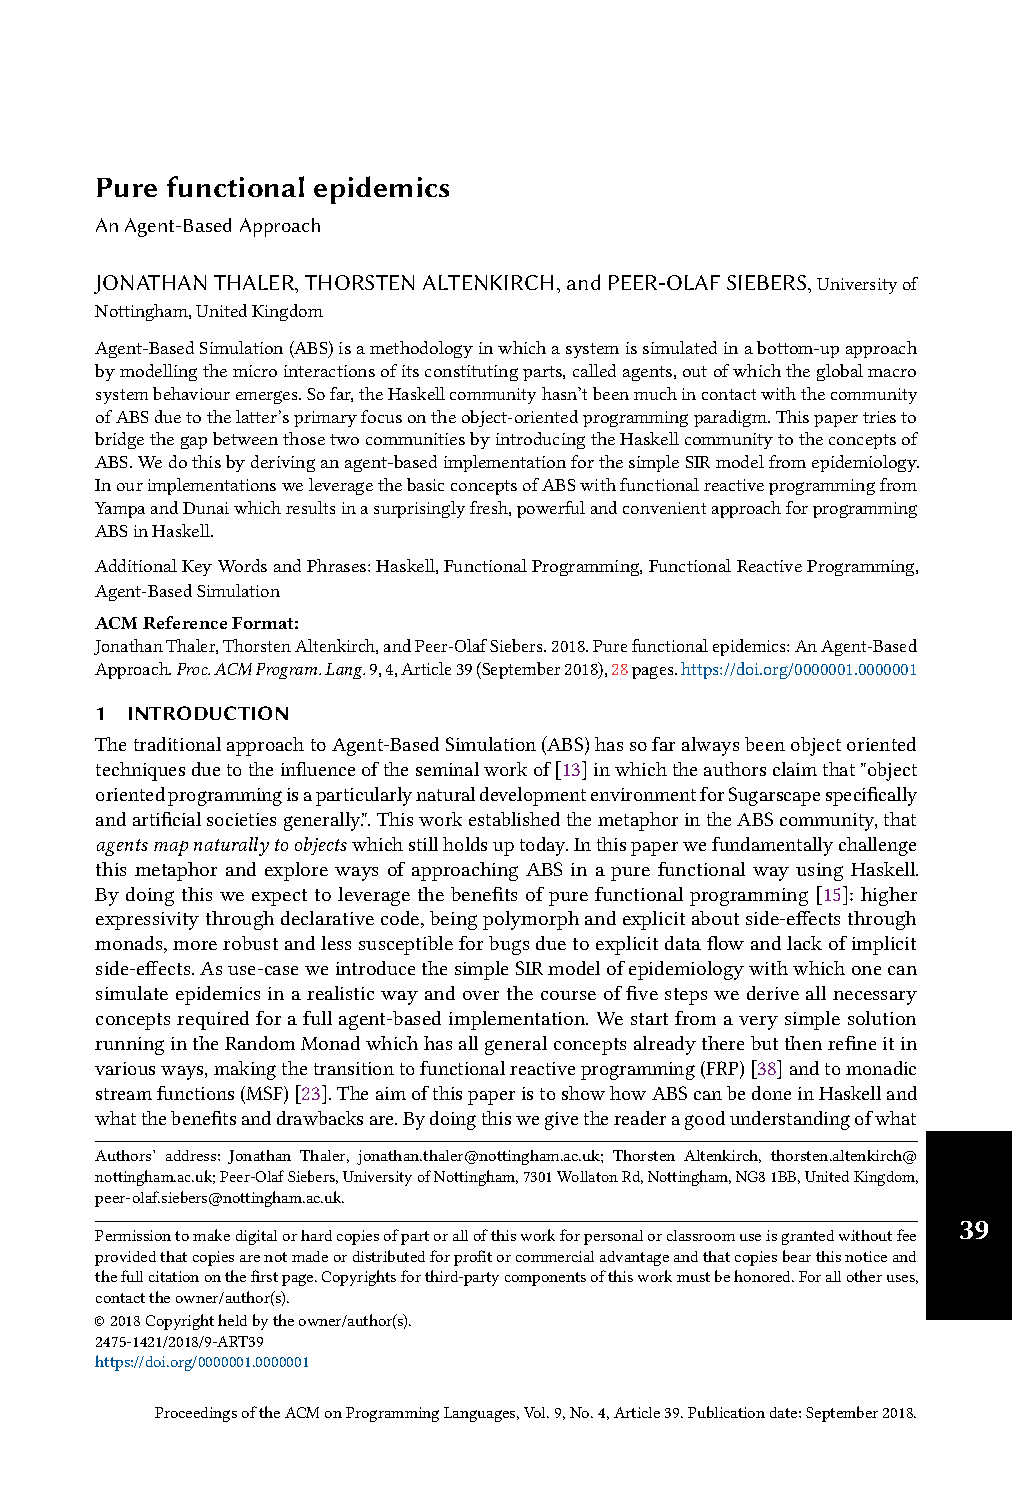
\includepdf[pages=-]{./pdf/pfe.pdf}

% NOTE: keep it out to the submission for the reviewers
%\chapter{Questions \& Answers}
\label{chap:qa}

TODO: update and adopt to 2nd year

In this chapter I give answers to anticipated questions and objections about my research direction and vision of doing pure functional ABS \footnote{They are not always posed in a dead-serious way but as it is a quite controversial topic - ABS should be done object-orientated after all huh? - I think it is appropriate. Also some objections were raised in exactly this way.}.

\paragraph{So you had this hypothesis, that pure functional programming and dependent types lead to simulation software which is more likely correct and is easier to verify and validate, right from the beginning?}
Not at all. I even had no deep knowledge of functional programming at the start of my PhD, I've just worked through the 1st edition of Grahams book "Programming in Haskell" and that's it. I had no clear understanding of purity, side-effects and Monads and I didn't know a bit about functional reactive programming. I knew that something like Dependent Types exist because Thorsten (2nd Supervisor) has sent me an email before the start of my PhD in which he pointed at Agda, so I started reading a bit about intuitionistic / constructivistic math, tried out a little bit of Agda but quickly gave up because it was way too far away (without really having mastered pure functional programming in Haskell, I believe it is nearly impossible / too difficult / makes no sense going into dependent types).
So in the beginning there was pure \textit{curiosity} about functional programming in combination with ABS because I knew nothing of FP at all and wanted to understand it (after getting bored by OO) and applying FP to ABS seemed so crazy (because everyone claims OO to be 'natural' for it) that it must be an extremely interesting challenge. I guess this is very often the case with research: there is 'just' curiosity in the beginning and then during the research process a hypothesis falls into place.


\chapter{Thesis Structure}
\label{app:thesis_struct}

TODO: find the story of my PhD thesis and connect it to my publication plan. 
TODO: story e.g. "We need functional programming to reduce the potential sources of bugs and introducing bugs harder, resulting in software which is more likely to be correct. Additionally by using dependent types we can narrow the gap between model specification and implementation even further, resulting in software which is even more likely to be correct. Further, additional benefits fall into place: purity leads to guaranteed reproducibility at compile-time, software transactional memory can be utilised to scale up to massively parallel and we have property-based testing at hand which puts the focus on specification testing rather than testing operational details".

This appendix gives a first draft of the structure outline of the thesis which I plan on start writing in April 2019. I aim for a flat structure which emphasises a strong narrative. The order of writing will be: Methodology, Proof-Of-Concept chapters, Literature Review, Discussion, Conclusions, Introduction, Abstract.
%
%line of argument
%1. established methods need extensive unit-testing for establishing correctness of software, which only increases the likelihood of correctness and doesnt guarantee it because they are inherent dynamic, testing run-time behaviour, because of the different type system.
%2. functional programming as in haskell has a strong static type system which allows to shift much much more guarantees towards static, compile-time, making many run-time tests obsolete and can guarantee a few things already at compile-time which makes tests to cover that completely obsolete
%3. dependent types can push these guarantees even further and theoretically should allow to express guarantees at compile-time to an arbitrary complex level which in theory should allow us to abandon run-time testing of bugs altogether. This does not mean that we don't need any tests anymore, as will be outlined in the chapter on Verification \& Validation \ref{chap:v_and_v}.
%4. with shifting more towards compile-time guarantees we automatically gain more confidence into the correctness of our simulation and reduce the implementation overhead of writing tests for those cases. Also some properties are simply not testable with run-time tests e.g. that some property holds forever - this is only possible to guarantee by looking at the code directly (where functional programming shines) or expressing it through compile-time guarantees. 
%5. correct by construction: narrowing the gap between model specification and implementation 
%6. Impedance Mismatch: ABS is constructive / generative in nature but the nature of the test-driven development process is deductive. is this a problem? Think of it more deeply


\section{Introduction}
This chapter is the introduction to the thesis and motivates it and describes the aim and scope of the Ph.D. Further it states the hypotheses and contributions.
\begin{itemize}
	\item Main Argument: Defining the problem, motivation, aim and scope of the Ph.D.
	\item Hypotheses: Precisely stating the hypotheses which will form the points of reference for the whole research.
	\item Contributions: Precisely list the contribution to knowledge this Ph.D. makes and list all papers which were written (and published) during this Ph.D.
\end{itemize}

\section{Literature Review}
This chapter discusses background and related work by presenting the relevant literature 

\section{Methodology}
This chapter introduces the methodology, used in the experimental chapters:

\begin{itemize}
	\item Defining and introducing Agent-Based Simulation (ABS) (History, ABS vs. MAS, examples, event- vs. time-driven).
	\item Introduce established implementation approaches to ABS (Frameworks: NetLogo, Anylogic, Libraries: RePast, DesmoJ, Programming: Java, Python, Correctness: ad-hoc, manual testing, test-driven development)
	\item Introduction Verification \& Validation (V \& V in the context of ABS).
	\item Introduction to functional Programming in Haskell (functions, types, recursion, algebraic data-types, higher-order functions, continuations, Define and explain side-effects and purity: monads, different types of effects, explain IO and that it is of fundamental importance to avoid it in our research).
	\item Introduction to dependent types (Example, Equality as Type, Philosophical Foundations: Constructive mathematics)
\end{itemize}

\section{Case Studies}
Presents case studies which are the main contribution of this Ph.D. which support our hypothesis. Each section is structured by Intro, Methods, Experiment, Analysis.

\subsection{Case Study 1: Testing and Verification}
This chapter describes how testing \& verification works in pure functional ABS.
%\begin{itemize}
%	\item Testing in functional programming
%	\item Strong Static Types rule out some classes of bugs and make some tests obsolete.
%	\item Property-Based testing: QuickCheck.
%	\item Using Property-Based testing in ABS for specification testing.
%	\item Reasoning about code
%\end{itemize}

\subsection{Case Study 2: Going Large-Scale}
This chapter discusses how pure functional ABS can go large-scale using STM. Further it is the central chapter, discussing various types of agent-agent and agent-environment interactions

%\subsubsection{Agent-Agent Interactions}
%This is the central problem of the FP approach as basically the agent-interactions define the level of abstractions over the agents. Unfortunately this is easier and more elegant in object-oriented programming. Still, by using a strong static type system we are more explicit about agent-interactions and we can have advantages which OOP doesn't have. Also we show that there are multiple different kinds of agent-interactions, depending on whether it is a time- or event-driven ABS.
%There is still much work to be done for this thesis chapter, we need to distinguish between:
%
%\begin{itemize}
%	\item Asynchronous Interaction: the flow is one-directional and does not need a listener on the other side and not a synchronous reply. The mechanism depends strongly on the type of ABS: time- or event-driven and pure or concurrent. Examples are the pure feedback in the Yampa SIR implementation, pure Data-Flow in the Yampa implementation, pure agent transactions, pure events, STM Event, STM message-boxes.
%	\item Synchronous Interactions: the flow is bi-directional and needs a listener on the other side to engage in a synchronous interaction without time-delay. We have only touched on prototyping this but need to go deeper for the final thesis. In Haskell we could build on the pure event driven approach we have implemented already in Step7\_EventDriven but we need to extend it towards an explicit synchronous mechanism. Also we need to show how we can do this in STM but there its gonna be very tricky because all agents act conceptually at the same time.
%\end{itemize}

\subsection{Case Study 3: Dependent Types}
This chapter gives an in-depth discussion on how dependent types can be made of use in pure functional ABS.

\section{Discussion}
This chapter re-visits the hypotheses and puts them into perspective of the contributions.

\section{Conclusions}
This chapter draws conclusions to the main hypothesis and outlines future research.

\section{Appendices}
Datasets, lengthy code, additional proofs.


\end{appendices}

\end{document}
